\chapter{Theory}
\label{cha:theory}
As mentioned in \autoref{cha:goals}, we want to understand the nature of the specific heat capacity of Copper. This requires an understanding of the underlying effects, that
influence the heat capacity. But it is more important to first understand what the heat capacity is. The Theory of the heat capacity will be discussed first in a calssical approach
and then in a qunantized approach. %this can be written better 
\section{Heat Capacity}
\label{sec:heat_capacity}
The heat capacity is defined as the amount of energy, which is needed to heat a body by $\qty{1}{\kelvin}$. That means the heat capacity is an amount of heat per temperature. The 
general formula is given by the equation \ref{eqn:heat_cap}, in which $\mathrm{d} Q$ is the needed amount of heat and $\mathrm{d} T$ is the temperature change.

\begin{equation}
    \label{eqn:heat_cap}
    C = \frac{\mathrm{d} Q}{\mathrm{d} T}
\end{equation} 

This definition of heat capacity leeds to a sample-size dependent quantity. Thus meaning a definition per $\mathrm{mol}$, per mass or per volume is more informative. The definition per $\mathrm{mol}$
is named \enquote{molar heat capacity}. The definition per mass and per volume is called \enquote{specific heat capacity}. They are distinguished via an index. To understand where the specific heat 
capacity is comming from, it is needed to approach this with thermodynamics. The first law of thermodynamics describes the energy balance of a system.
\begin{equation}
    \label{eqn:first_hs}
    \mathrm{d}E = \mathrm{d} Q + \mathrm{d} W = T\mathrm{d}S - p\mathrm{d}V
\end{equation}

In equation \ref{eqn:first_hs} it can be seen, that $\delta W = 0$ for a constant volume, because $\mathrm{d}V = 0$. Applying this information to equation \ref{eqn:heat_cap} it yields
that for constant volume the specific heat capacity can be described by the following equation \ref{eqn:heat_cap_v}.

\begin{equation}
    \label{eqn:heat_cap_v}
    C_{\mathrm{V}} = \left.\frac{\partial E}{\partial T} \right\vert_\mathrm{V}
\end{equation}

To get the specific heat capacity for a constant pressure, we have to apply an legendre transformation to the energy. This transformation leeds to the enthalpy $H$ given by equation \ref{eqn:enthalpy}.
The enthalpy $H$ is, similar to the inner energy $E$, a measure of energy in an thermodynamic system.

\begin{equation}
    \label{eqn:enthalpy}
    \mathrm{d}H(S,p,N) = \mathrm{d}E(S,V,N) + p\mathrm{d}V + V\mathrm{d}p = T\mathrm{d}S - p\mathrm{d}V + p\mathrm{d}V + V\mathrm{d}p = T\mathrm{d}S + V\mathrm{d}p
\end{equation}

Using $p =$ const this equation yields $\mathrm{d}H = \mathrm{d}Q$. Adding this to the definition of the specific heat capacity results in equations \ref{eqn:state_func} describing the specific 
heat capacity with a fitting thermodynamic state functions.
\begin{equation}
    \label{eqn:state_func}
    C_\mathrm{V} = \left.\frac{\partial E}{\partial T} \right\vert_\mathrm{V} \,\,\,,\,\,\, C_\mathrm{p} = \left.\frac{\partial H}{\partial T} \right\vert_\mathrm{p}
\end{equation}

\section{Comparisson of $C_\mathrm{V}$ and $C_\mathrm{p}$}
From measurements it is known, that $C_\mathrm{V}$ and $C_\mathrm{p}$ differ to some extend. The reason for this is, that for a constant pressure $p$ the volume $V$ of the sample 
changes, thus work has to be put into the deformation of the solid. This creates a loss of energy that does not exist for a constant volume. This is an isentropic process, therefore 
the adiabat equation is valid. The isentropic constant, which is given by $\kappa = \frac{C_\mathrm{p}}{C_\mathrm{V}}$, describes the ratio of the two specific heat capacities. It can 
be approximated by equation \ref{eqn:isentropic_const_dof}, in which f is the amount of dof. 

\begin{equation}
    \label{eqn:isentropic_const_dof}
    \kappa = \frac{f+2}{f}
\end{equation}

For a solid in a classical approach(6 dof), this yields an ratio $\kappa = \frac{4}{3}$. This ratio is larger than one, therefore $C_\mathrm{p} > C_\mathrm{V}$.
This difference in these two seemingly similar quantities, not at all random. More so it is thightly embedded in thermodynamic theory. At this point the derivation of the correction 
formula is not shown. The correction formula is given by equation \ref{eqn:p_v_correction}.

\begin{equation}
    \label{eqn:p_v_correction}
    C_\mathrm{p} - C_\mathrm{V} = 9\alpha^2\kappa V_0T
\end{equation}

$\alpha$ being the thermal expansion coefficient, $\kappa$ the bulk modulus, $V_0$ the molar volume and $T$ the temperature.

\section{Classical Theory of the Heat Capacity}
\label{sec:classical}
In \autoref{sec:heat_capacity} the formula for the specific heat capacity with constant volume was derived. Thus $C_\mathrm{V}$ is dependent on the inner energy of a system. To 
calculate the inner energy it is of interest to understand what defines or gives an solid state sample inner enregy. The answer is lattice vibrations. For each of the three directions
in space, there are two possible vibration modes. Thus having a three dimensional sample, there are six degrees of freedom(\enquote{dof}). To compare this an ideal gas has three (kinetic)
dof.

The equipartition theorem states, that every
dof has an energy of $\frac{1}{2}k_\mathrm{B}T$. $k_\mathrm{B}$ is the boltzmann-constant and $T$ the temperature. With this it is possible to calculate the \enquote{classical} inner
energy of an sample as shown in equation \ref{eqn:inner_E_clas}.

\begin{equation}
    \label{eqn:inner_E_clas}
    E = N_{\mathrm{dof}}^{'} N_{\mathrm{atoms}} \frac{1}{2}k_\mathrm{B}T = \frac{6}{2}k_\mathrm{B}T = 3k_\mathrm{B}T
\end{equation}

Now the specific heat capacity can be calculated using equation \ref{eqn:heat_cap_v}, which results in \ref{eqn:dulong_petit}.

\begin{equation}
    \label{eqn:dulong_petit}
    C_\mathrm{V} = 3Nk_\mathrm{B}
\end{equation}

This is the \enquote{Law of Dulong-Petit}, which describes the classical limit of the specific heat capacity. Note, that the calssical limit is not dependent on the temperature.

\section{Experimental partially falsification of the Law of Dulong-Petit}
\label{sec:ueberleitung}
Now that we have a model for the temperature-dependece of the specific heat capacity, we can compare the model to measured data, to evaluate the theoretical model. For this a temperature
measurement of the heat capacity is needed. In \autoref{fig:heat_cap_measurement} we can see, that $C_\mathrm{p}$ is not constant in temperature. From this follows, that $C_\mathrm{V}$
is also not constant in temperature, since the difference between $C_\mathrm{p}$ and $C_\mathrm{V}$ is small in a solid.

\begin{figure}
    \centering
    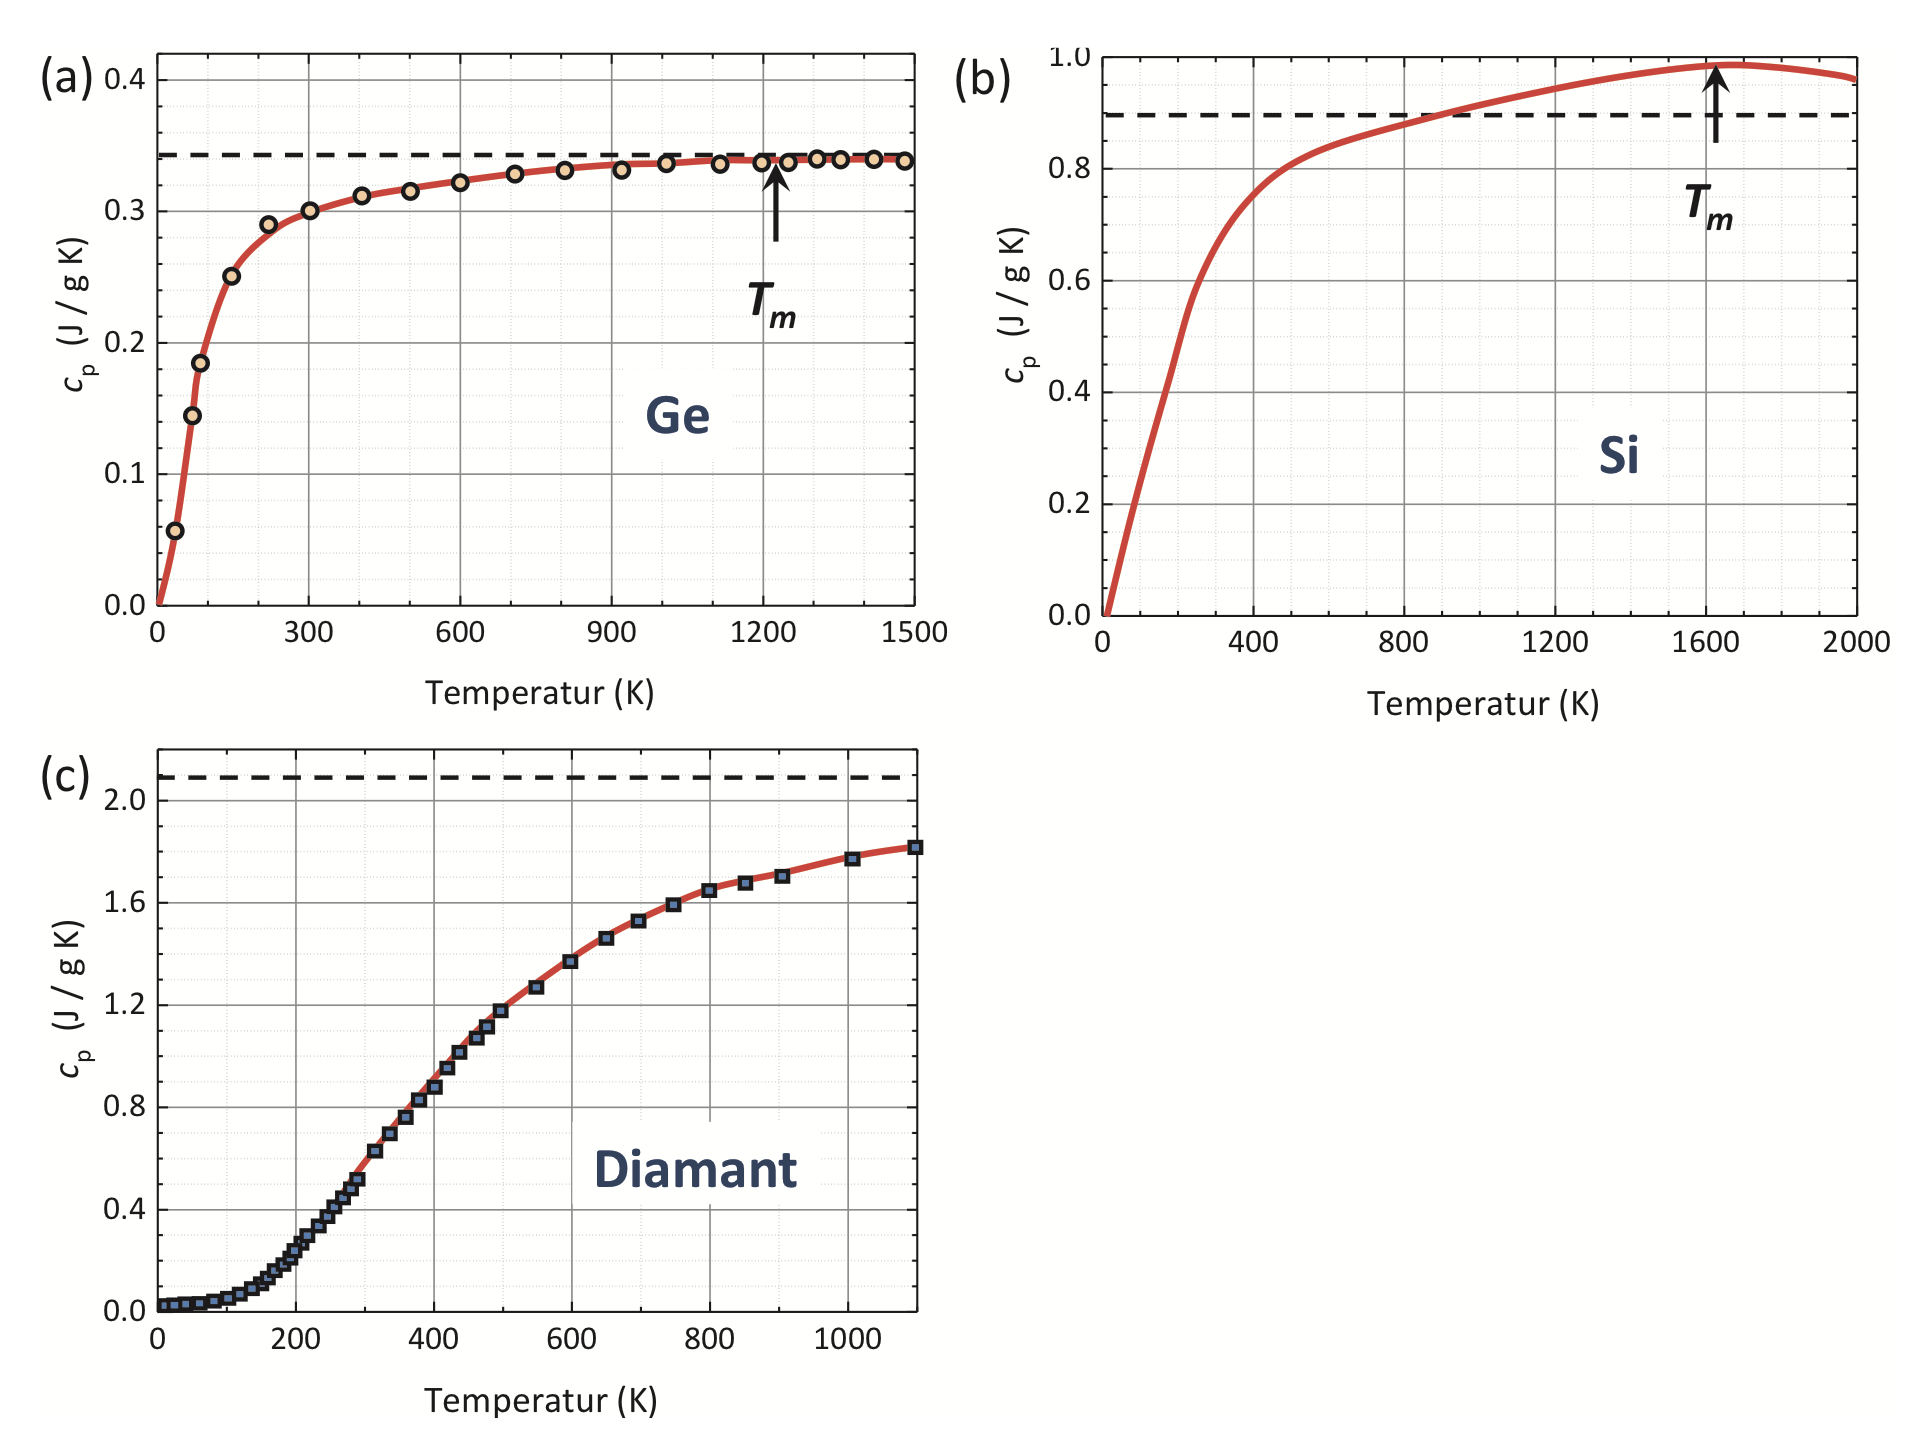
\includegraphics[scale=0.4]{content/V47_pictures/heat_capacity.png}
    \caption{In this figure we can see the temperature-dependece of the specific heat capacity $C_\mathrm{p}$ for different solids. \cite{grossmarx}}
    \label{fig:heat_cap_measurement}
\end{figure}

From the measurement, we can see that the classical limit, which means for high temperatures, the Dulong-Petit law is valid. Small deviations come due to anharmonic effects dominating
for higher $T$. But the significant perception is, that for low temperatures $C_\mathrm{V} \propto T^3$. Therefore \enquote{new physics} must be the explaination. With the idea of qunantization
of classically continuous phenomena a new idea for the calculation of the inner energy in a solid state system came up.

\section{Quantummechanical Theory of the Heat Capacity}
\label{sec:quantum}
Now we want to look at a quantized nature of lattice vibrations, so called \textit{Phonons}. Even so the Dulong-Petit model cannot describe the heat capacity for low temperatures, the approach over the energy 
lattice vibrations is not incorrect. If we describe the vibrations not as classcial oscillators, but as quantummechanical oscillators. Therefore the states in the low temperature regime 
are quantized, because $\hbar\omega >> k_\mathrm{B}T$.
%kurze liste für reihenfolge der themen
%sec:übergang zu quantenmechanischer betrachtung, phononen dispersion und allg innere energie def
%sec:einsteinnäherung
%sec:Debye näherung